\documentclass[11pt]{article}
\usepackage[margin=1.0in]{geometry}

% Required packages
\usepackage{amsmath,amsfonts,amsthm,amssymb} % Mathematical typesetting and symbols
\usepackage{bigstrut} % Row spacing
\usepackage{enumerate} % Custom enumerate labels
\usepackage{esint} % Alternate double integral symbols
\usepackage{fancyhdr} % Headers and footers
\usepackage{graphicx} % Figure inclusion
\usepackage{hyperref} % Hyperlinks for citations, references, and URLs
\usepackage{placeins} % Float barriers
\usepackage{slashbox} % Slash in a table cell
\usepackage{subcaption} % Captions for subfigures
\usepackage{titlesec} % Custom section labels
\usepackage{wrapfig} % Wrapping text around figures
\usepackage{xcolor} % Text color

% Label Sections as Parts
\titleformat{\section}{\normalfont\Large\bfseries}{Part \thesection:}{0.5em}{}

% Define license image
\newcommand{\licenseimage}{figures/by-sa.png}

% Footer for first page
\pagestyle{plain}
\renewcommand{\headrulewidth}{0pt}
\fancyhead{}
\fancyfoot{}
\cfoot{\includegraphics[width=0.75in]{\licenseimage} \\ \footnotesize This work by the \href{https://floridapoly.edu/academic-departments/applied-mathematics.php}{Department of Applied Mathematics at Florida Polytechnic University} is licensed under a \href{https://creativecommons.org/licenses/by-sa/4.0/}{Creative Commons Attribution-ShareAlike 4.0 International License}.}


%==============================================================================

\begin{document}

\noindent \makebox[\textwidth]{\textbf{\LARGE \textcolor{red}{Title}}}

\quad

%% Update cover image
\begin{figure}[h]
	\centering
	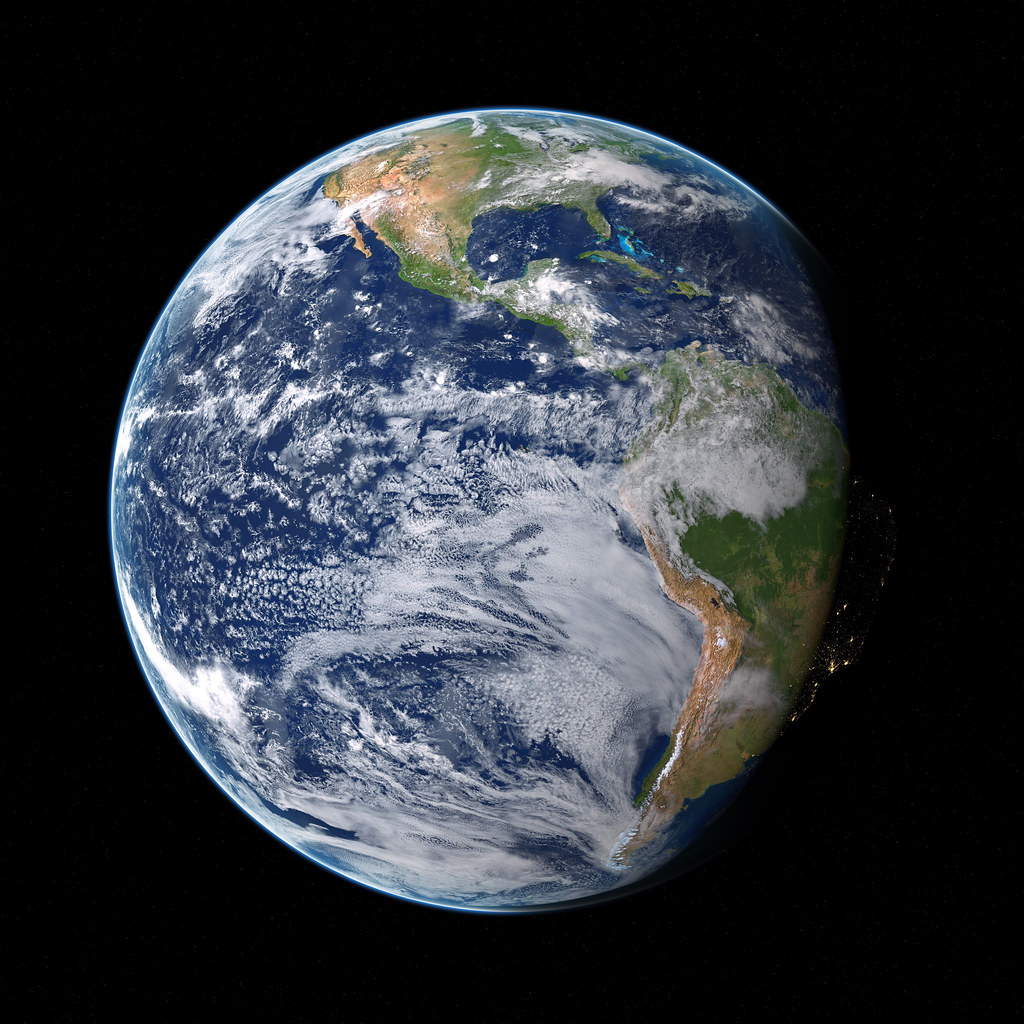
\includegraphics[width=0.45\textwidth]{figures/earth.jpg}
\end{figure}

%==============================================================================
\section*{Introduction}

\thispagestyle{fancy} % Add footer to first page only

\textcolor{red}{Introductory paragraphs}

%%%
\subsection*{Learning Objectives}

After completing this project, you should be able to:
\begin{itemize}
	\item \textcolor{red}{List of learning objectives}
\end{itemize}

%==============================================================================
\section{\textcolor{red}{Section Title}}
\label{sec:sectiontitle}

\textcolor{red}{Section description}

%%%
\subsection*{Activity}

\textcolor{red}{Activity introduction}

\begin{enumerate}[\bf {\thesection}a.]
	\item \textcolor{red}{Parts of activity}
\end{enumerate}

\end{document}
